\chapter{线缺陷}
    \section{位错概念的引入}
        \subsection{实际晶体的滑移特征}
            在早期对金属材料的范性形变\index{范性形变}的研究中发现:
            \begin{itemize}
                \item[1] 单晶体发生范性形变时表面出现小台阶滑移线;
                \item[2] 晶体滑移总是沿着一定的密排晶面和密排方向,而且只有沿着这些面和方向的切应力达到一个临界值时,滑移才开始进行。
            \end{itemize}
            对与金属单晶来说,这个临界值在\SIrange{1}{10}{\MPa}。在这种情况下,人们引入晶体的理想模型来解决这个问题。

        \subsection{理想晶体的滑移}
            为了解释晶体的变形现象,人们提出了刚性滑移假设\index{刚性滑移假设}。
            假设滑移时滑移面两端的晶体为刚体,原子同步平移,设$T$为加载在晶体上的切应力,在缓慢变形中,该应力与变形相平衡。
            应力大小随滑移面两侧晶体相对位移量变化。

            由于晶体排列具有周期性,点阵对滑移的阻力也是周期性的,变形过程如\autoref{理想晶体变形示意图}所示,
            \begin{figure}[ht]
                \centering
                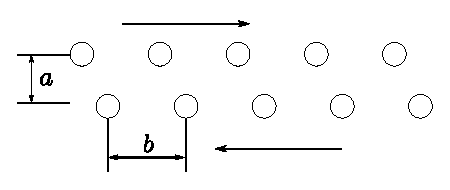
\includegraphics[width=0.7\textwidth]{fig/理想晶体变形示意图.eps}
                \caption{理想晶体变形示意图。}
                \label{理想晶体变形示意图}
            \end{figure}
            
            假定变形所受到的阻力为
            \begin{equation}
                \tau=\tau_m\sin{\left( \frac{2\pi x}{b} \right)}
            \end{equation}
            当发生的变形很小时,可以近似为
            \begin{equation}
                \tau=\tau_m{\left( \frac{2\pi x}{b} \right)},
            \end{equation}
            而且开始变形时,晶体处于弹性阶段,应当满足虎克定律,也就是
            \begin{equation}
                \tau=\mu\gamma=\mu\frac{x}{a},
            \end{equation}
            其中$\mu$为切变模量,$\gamma$为切应变,因此可以得到最大切应力为
            \begin{equation}
                \tau_m=\frac{\mu b}{2\pi a},
            \end{equation}
            由于本课程讨论的晶体绝大多数情况为简单立方晶系,可以认为$a=b$,所以最大切应变为
            \begin{equation}
                \tau_m=\frac{\mu}{2\pi}.
            \end{equation}

            然而理论切变强度$\frac{\mu}{2\pi}$与实际强度相比,实在太大。在使用更为合适的原子间作用力模型后,改变了正弦近似,
            最大切应变数值上降低为原来的$1/60$,但是这仍然比实际值高出了3到4个数量级。

            然而无论如何都提高应力模型的精确程度,最终结果的偏差仍然很大,因此是假设出现了问题。最终人们提出了位错模型,并且在
            实验中观察到了这一现象。
        
        \section{位错的结构}
            晶体中存在三种不同的位错类型,下面将分别描述。
            \subsection{刃型位错}
                考虑一个简单立方晶体,它在$(010)$面上沿$[100]$方向发生滑移,但是这个滑移是不均匀的。
                也就是从晶体的右侧向左传播。在某一时刻,滑移停止在晶体内部。于是在这个$(010)$面左右就可以划分出已滑移区域和未滑移区域,
                该面也就是两个区域的边界。晶体滑移的元过程是在一定的晶体学面上,沿一定的晶体学方向,晶体的上下两部分相对滑移一个或着多个
                点阵常数的距离。

                由此显然可见,已滑移的地区与未滑移的地区是一样的,上述滑移平面上下原子列是恢复对齐的,也就是说,这些地方恢复了理想晶体的长程
                有序性。所以除去\autoref{刃型位错形成示意图}中$\perp$的位置外,晶体的其他部分都是完整的。在这一区域内,晶体的完整周期性显然被
                破坏,所以这就是一个晶体缺陷,称为位错\index{位错}。
                \begin{figure}[ht]
                    \centering
                    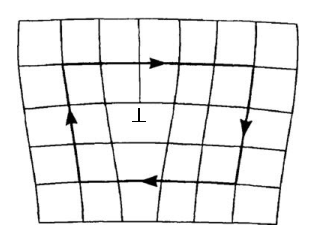
\includegraphics[width=0.45\textwidth]{fig/刃型位错示意图b.eps}
                    \caption{刃型位错形成示意图。}
                    \label{刃型位错形成示意图}
                \end{figure}

                关于位错最为简单的定义就是:位错是近完整晶体中的一个缺陷,是晶体中已滑移区和未滑移区的边界。
                
                这个边界更为严格的说,是分界区域的中心轴线,是平行于$[011]$方向的一条直线,其与滑移矢量$[100]$垂直,那么
                这个位错就称为刃型位错。

                上述中心轴线称为位错线\index{位错线},原理位错线的区域保持理想晶体的完整性;只有极为接近位错线的区域,也就是上述分界区域或
                过渡区域,晶体的点阵结构,或者原子的规则排列被破坏这一区域称为位错核心\index{位错!位错核心}。位错核心的半径与位错线的长度
                相比非常小,所以说,位错是晶体中的线性缺陷。

                对于刃型位错\index{位错!刃型位错},其与滑移矢量垂直,而\autoref{刃型位错形成示意图}中,$\perp$符号代表多余的一个半原子面,
                这个半原子面的边缘就是刃型位错的位错线,形状类似刀刃,因此称为刃位错\index{位错!刃位错}。
                因此刃型位错的形成也可以认为是一个半原子面中断与晶体内部,该边缘也就是一个刃型位错。

                在规定分割面的上下后,半原子面在割面上方的位错称为正刃型位错,反之则为负刃型位错,但是两者并没有本质上的区别。

                刃型位错有以下结构特点
                \begin{itemize}
                    \item[1] 位错周围有弹性畸变或非弹性畸变,上半部分晶体受压力,下部分受张力,中心为最大畸变,畸变局限在2或3个原子间距的管道内,总体为线缺陷;
                    \item[2] 位错线与滑移方向垂直;
                    \item[3] 上下晶体有一个相对位移$\vec{b}$,称为伯格斯矢量或简称柏式矢量\index{柏式矢量}。
                \end{itemize}
            \subsection{螺型位错}
                仍然假定滑移面为$\left( 010 \right)$面,位错线仍然是沿$[001]$方向的直线,但是滑移方向变为$[001]$方向,
                即为与位错线平行的方向,仍然将晶体分为已滑移区、未滑移区以及中间的过渡地带。同样,整个晶体是近完整的,只有在位错核心区,晶体的点阵
                结构才遭到破坏。
                
                也就是说,这也是一个二维缺陷,但是原子排列方式与刃型位错却不相同,不难得出,对与位错线垂直的原子面
                在位错不存在时,是一组彼此平行分立的平面,当此位错存在时,他们则变成一个连续的螺旋面。
                若绕此位错线以左手螺旋正向环行一周,即从一个面上升到相邻的另一个原子面,由于这个形质,这种位错称为螺型位错\index{位错!螺位错}。
                
                \begin{figure}[ht]
                    \centering
                    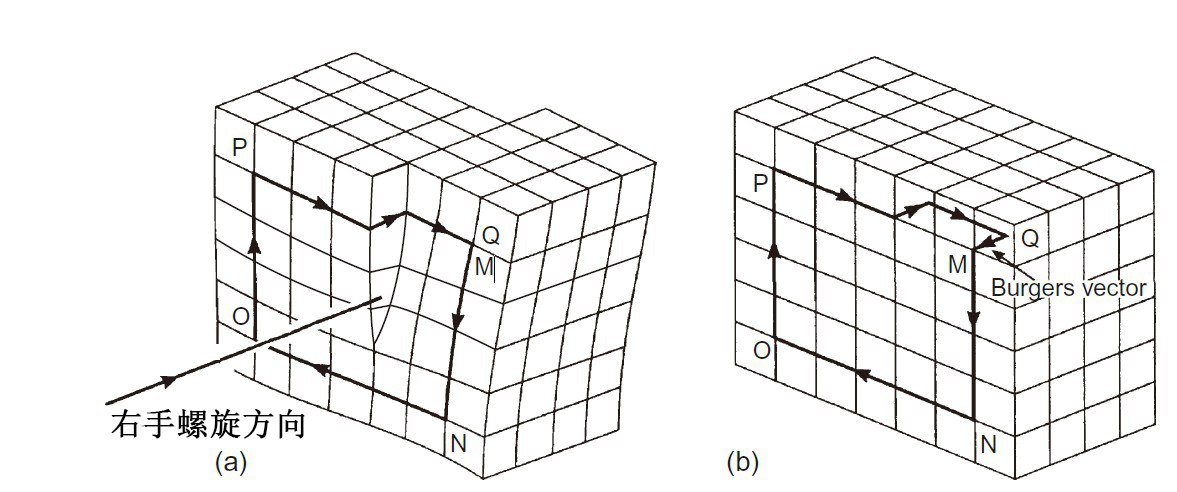
\includegraphics[width=0.7\textwidth]{fig/螺型位错示意图.jpg}
                    \caption{左螺型位错示意图,(a)螺型位错的左手螺旋回路,(b)为相同回路在理想晶体中的绕行状况。}
                    \label{螺型位错示意图}
                \end{figure}

                在规定位错线正方向后,若绕位错线以右手螺旋方向绕行一周后,可以上升一个原子面的位错为右螺型位错,
                若绕位错线以左手螺旋方向绕行一周后,可以上升一个原子面的位错为左螺型位错,如\autoref{螺型位错示意图}。
                左螺型位错和右螺型位错的滑移矢量方向也是相反的。

                在含有螺型位错的晶体中,原子面排布如\autoref{右螺型位错原子面排布}所示。晶体不再是刃型位错的附加半原子面,而是变成了螺旋式的曲面。
                \begin{figure}[ht]
                    \centering
                    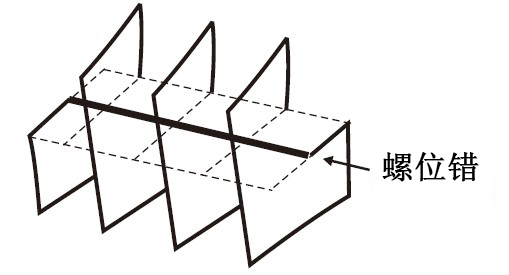
\includegraphics[width=0.5\textwidth]{fig/螺位错原子面排布.jpg}
                    \caption{右螺型位错原子面排布。}
                    \label{右螺型位错原子面排布}
                \end{figure}
            \subsection{混合型位错}
                然而一根直线位错可能既不与滑移矢量$\vec{b}$垂直,也不平行,而是成一个角度$\theta$,则这个位错既不是纯刃型位错也不是纯螺型位错,
                它可以看作是两个直线位错的叠加,分别为纯刃型和纯螺型的位错,两者的滑移矢量大小为
                \begin{align}
                    \vec{b}_1=\vec{b}\sin\theta,\\
                    \vec{b}_2=\vec{b}\cos\theta.
                \end{align}
                这个直线位错称为混合位错\index{位错!混合位错}。组成混合位错的两个分量为刃型分量和螺型分量。

                对上述情况加以推广,假设滑移矢量为$\vec{b}$,已滑移区域为\autoref{混合型位错的滑移示意}中的阴影部分,而位错线为图中红色线,从垂直与滑移面的方向看去,上下两个原子
                面之间的原子排布应该为\autoref{混合型位错的原子排列示意图}所示。
                \begin{figure}[ht]
                    \centering
                    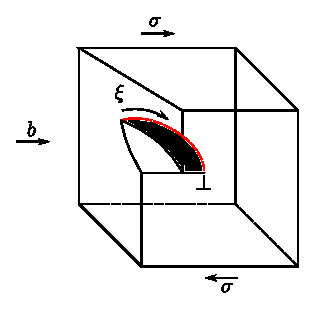
\includegraphics[width=0.5\textwidth]{fig/混合型位错的滑移示意.eps}
                    \caption{混合型位错的滑移示意。}
                    \label{混合型位错的滑移示意}
                \end{figure}
                
                \begin{figure}[ht]
                    \centering
                    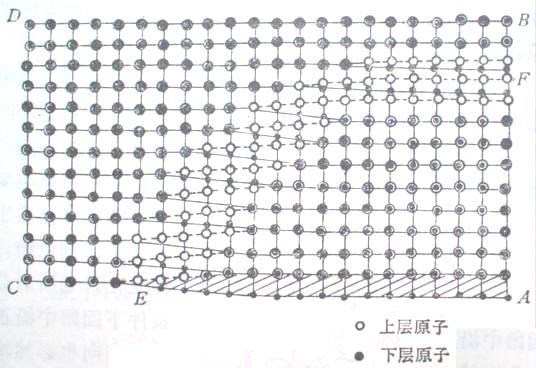
\includegraphics[width=0.5\textwidth]{fig/混合型位错的原子排列示意图.jpg}
                    \caption{混合型位错的原子排列示意图。}
                    \label{混合型位错的原子排列示意图}
                \end{figure}
                从\autoref{混合型位错的原子排列示意图}可以看出,这个位错有一段是纯螺型位错,另一端是纯刃型位错,由于位错线是连续的\footnote{这一点需要会证明。}
                从晶体的一个表面延伸到另一个表面,中间弯曲的一端既不是螺型位错也不是刃型位错,而是同时具有螺型和刃型位错的特征。
                这一小段也可以看作是许多方向近连续变化的小直线段所组成,每一小段都是混合型位错,各有一个螺型分量和刃型分量。
            \subsection{小结}
                依照以上定义,位错是晶体中滑移面上两个区域(即已滑移区域和未滑移区域)之间的分界,那么它就应该具有两个重要的性质:
                \begin{itemize}
                    \item[1] 因为晶体的滑移矢量是一个恒定矢量,等于一个或多个最小点阵平移矢量,所以对于一条位错线的各个部分,滑移矢量均相等;
                    \item[2] 无论位错线形状如何,总之位错线绝不可能终止于晶体的内部,位错线只能从晶体的一个表面延伸到另一个表面,或是在晶体中形成一个封闭的环。
                \end{itemize}
        \section{位错的普遍定义与伯格斯矢量}
            \subsection{位错的普遍定义}
                